\documentclass[border=10pt]{standalone}
\usepackage{xcolor}
\usepackage{pgfplots}
\usepackage{tikz}
\begin{document}
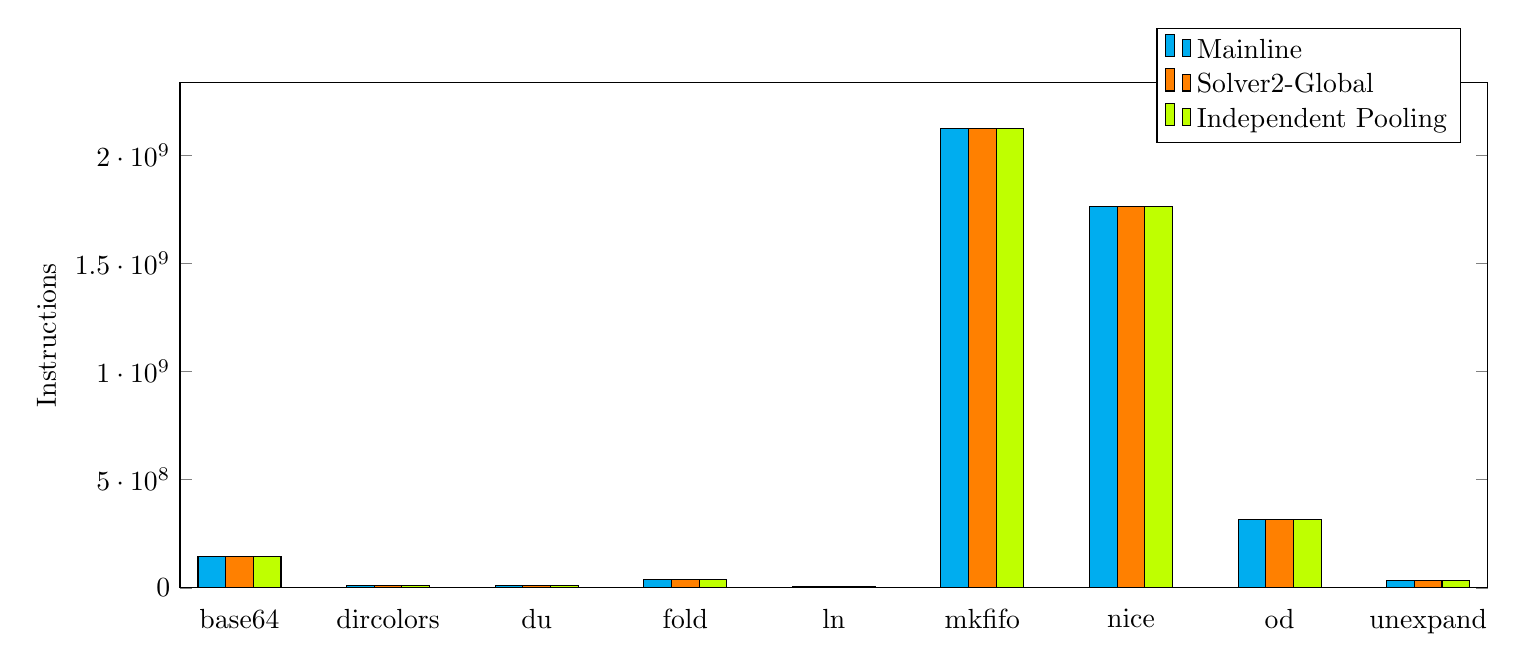
\begin{tikzpicture}
    \begin{axis}[
        width  = 1.5 * \textwidth,
        height = 8cm,
        major x tick style = transparent,
        % tickwidth=10,
        ybar=0,
        bar width=10pt,
        % ymajorgrids = true,
        ylabel = {Instructions},
        symbolic x coords={base64,dircolors,du,fold,ln,mkfifo,nice,od,unexpand},
        xtick = data,
        scaled y ticks = false,
        enlarge x limits=0.05,
        ymin=0,
        legend cell align=left,
        legend style={
                at={(0.98,0.88)},
                anchor=south east,
                % column sep=1ex
        }
    ]
        \addplot[style={cyan,fill=cyan,mark=none}, draw=black]
	coordinates {(base64,143698238) (dircolors,10858522) (du,10912153) (fold,36998646) (ln,6355212) (mkfifo,2122518592) (nice,1763019281) (od,316558102) (unexpand,34456067)};
\addplot[style={orange,fill=orange,mark=none}, draw=black]
	coordinates {(base64,143698238) (dircolors,10858522) (du,10912153) (fold,36998646) (ln,6355212) (mkfifo,2122518592) (nice,1763019281) (od,316558102) (unexpand,34456067)};
\addplot[style={lime,fill=lime,mark=none}, draw=black]
	coordinates {(base64,143698238) (dircolors,10858522) (du,10912153) (fold,36998646) (ln,6355212) (mkfifo,2122518592) (nice,1763019281) (od,316558102) (unexpand,34456067)};

        \legend{Mainline,Solver2-Global,Independent Pooling}
    \end{axis}
\end{tikzpicture}
\end{document}
